\documentclass[10pt]{article}

\usepackage[utf8]{inputenc}
\usepackage{amsmath, amssymb, amsfonts, amsthm}
\usepackage{upgreek}
\usepackage{amsthm}
\usepackage{fullpage}
\usepackage{graphicx}
\usepackage{cancel}
\usepackage{subfigure}
\usepackage{mathrsfs}
\usepackage{enumerate}
%\usepackage{outlines}
\usepackage[font={sf,it}, labelfont={sf,bf}, labelsep=space, belowskip=5pt]{caption}
\usepackage{hyperref}
% \usepackage{minted}

\usepackage{float}
% \floatplacement{figure}{H}

\usepackage{fancyhdr}
\usepackage[title]{appendix}
\usepackage{siunitx}

\DeclareMathOperator{\tr}{tr}
\DeclareMathOperator{\sgn}{sgn}
\DeclareMathOperator{\sinc}{sinc}
\DeclareMathOperator{\rref}{rref}
\DeclareMathOperator{\cof}{cof}

\pagestyle{fancy}
\headheight 24pt
\headsep    12pt
\lhead{}
\fancyfoot[C]{} % hide the default page number at the bottom
\lfoot{}
\rfoot{\thepage}
\renewcommand{\headrulewidth}{0.4pt}
\renewcommand\footrulewidth{0.4pt}
\providecommand{\abs}[1]{\lvert#1\rvert}
\providecommand{\norm}[1]{\lVert#1\rVert}
\providecommand{\dx}{\, \mathrm{d}x}
\providecommand{\dA}{\, \mathrm{d}A}
% \providecommand{\vint}[2]{\int_{#1} \! #2 \, \mathrm{d}x}
% \providecommand{\sint}[2]{\int_{\partial #1} \! #2 \, \mathrm{d}A}
\renewcommand{\div}{\nabla \cdot}
\providecommand{\e}{\epsilon}
\providecommand{\shape}{\Omega(p)}
\providecommand{\boundary}{\partial \shape}
\providecommand{\vint}[1]{\int_{\shape} \! #1 \, \mathrm{d}x}
\providecommand{\sint}[1]{\int_{\boundary} \! #1 \, \mathrm{d}A}
\providecommand{\pder}[2]{\frac{\partial #1}{\partial #2}}
\providecommand{\tder}[2]{\frac{\mathrm{d} #1}{\mathrm{d} #2}}
\providecommand{\evalat}[2]{\left.#1\right|_{#2}}
\newcommand{\defeq}{\vcentcolon=}
\newtheorem{lemma}{Lemma}
\newcommand\numberthis{\addtocounter{equation}{1}\tag{\theequation}}

\makeatletter
\usepackage{mathtools}
\newcases{mycases}{\quad}{%
  \hfil$\m@th\displaystyle{##}$}{$\m@th\displaystyle{##}$\hfil}{\lbrace}{.}
\makeatother
\DeclarePairedDelimiter\ceil{\lceil}{\rceil}
\DeclarePairedDelimiter\floor{\lfloor}{\rfloor}

\newenvironment{amatrix}[1]{%
  \left[\begin{array}{@{}*{#1}{c}|c@{}}
}{%
  \end{array}\right]
}

\title{Periodic Homogenization of Elasticity Tensors}
\author{Julian Panetta}

% BEGIN DOCUMENT
\begin{document}

\maketitle
    \begin{figure}[H]
        \centering
        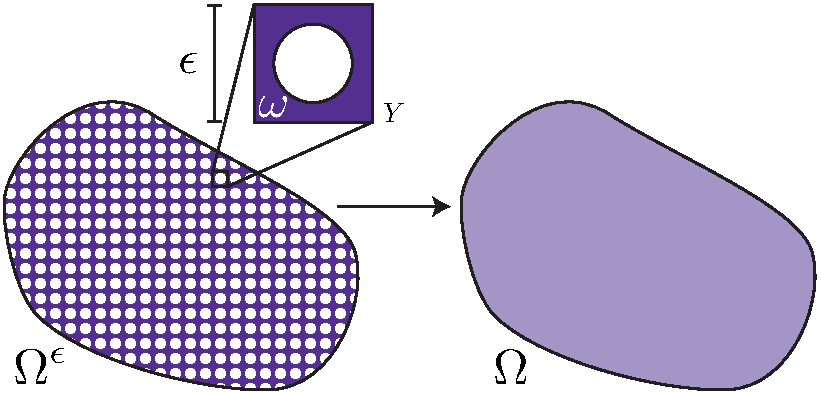
\includegraphics[width=.75\textwidth]{Images/homogenize.pdf}
        \caption{Base cell geometry $\omega$ is tiled with period $\epsilon$
            throughout $\Omega$ to get a porous, microstructured object
        $\Omega^\epsilon$. As $\epsilon \to 0$, $\Omega^\epsilon$ behaves
        identically to a solid version of $\Omega$ filled with
        ``homogenized'' material $C^H$.}
        \label{fig:homogenization}
    \end{figure}
\section{Introduction}
In solid mechanics, we model objects as continua. That is,
we assume that the size of an object is large enough that we needn't consider
its individual molecules and their interactions. We instead capture the
effect of all these microscopic scale interactions using a constitutive
relation, describing how much force is required to stretch an infinitesimal
piece of the object in each possible way. This relationship is determined by the
material of the object, which is formalized as the rank 4 ``elasticity'' (or
``stiffness'') tensor field, $C_{ijkl}$.

But what if the object is porous or a fine-scale composite of
multiple materials? Can we apply the same assumptions at a larger length scale
to still model the object as a solid, homogeneous continuum? It turns out that
we can, and homogenization theory gives a rigorously justified method to do
it.

\subsection{Motivation}
There are several situations where the homogenization-based modeling approach
is desirable. First, it is a more tractable model for numerical simulation,
e.g. via the finite element method. With homogenization, the computation mesh
no longer has to resolve all the fine microstructure of $\Omega^\e$. This means
a much coarser mesh with fewer degrees of freedom can be used, resulting in
smaller linear systems after discretization. Second, the homogenized material
properties themselves give us a lot of information about a pattern. For example,
a microstructure's homogenized Young's modulus in a particular direction tells
us how hard we must pull on a block-shaped tiling of the structure to stretch
it--no numerical simulation required!

Another motivation comes from microstructure design and fabrication. With the
recent advances in 3D printers, it is now possible to fabricate complicated
geometry rapidly and at low cost. However, the printer materials are somewhat
limited and typically cannot vary across an object. So, if we want to print,
say, an action figure that bends at the joints but is stiff elsewhere, we must
achieve this effect by varying the geometry. This goal leads us to consider the
inverse problem: designing a printable microstructure that has some desired
effective behavior. The inverse problem can be formulated as an optimization
problem whose objective is a function of the homogenized material properties.
The prerequisite for solving such a problem is, of course, finding these
material properties.

\section{Periodic Homogenization}
Our goal is to find the homogenized elasticity tensor $C^H_{ijkl}$,
which tells us the effective properties of the microstructure when it is
fabricated at a small enough scale. That is, if we fabricate a solid version of
$\Omega$ filled with $C^H$, it will deform identically to $\Omega^\e$ for small
enough $\e$.

A natural question to ask is: why not just spatially
average $C_{ijkl}({\bf y})$ over the microstructure? But it is clear from the
1D case why this would give the wrong answer: consider two equal-length springs
connected in series with very different spring constants $k_1 \ll k_2$. The
spatial averaging approach is equivalent to saying that the effective spring
constant of the coupled springs is $.5 (k_1 + k_2)$. However, the true
effective spring constant will be much closer to $k_1$ than to the average
(indeed, it is the harmonic mean of $k_1$ and $k_2$).

\begin{figure}
    \centering
    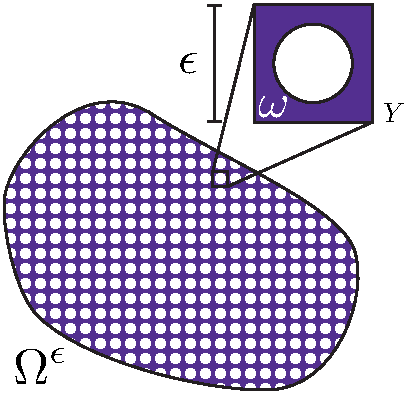
\includegraphics[width=.35\textwidth]{Images/periodic.pdf}
    \caption{Periodic tiling of base cell $Y$ with geometry $\omega$ throughout
    domain $\Omega$ and length scale $\e$.}
    \label{fig:periodic}
\end{figure}

\subsection{Framework}
We simplify the problem by considering only periodic microstructures (Figure
\ref{fig:periodic}). This means that our microstructured object, $\Omega^\e$,
is given by tiling $\Omega$ with base cell geometry $\omega$ contained in cell $Y$.
Parameter $\epsilon$ determines the size of cell $Y$, so the smaller $\epsilon$
gets, the more repetitions of $\omega$ are fit into $\Omega$, and the closer we
get to a homogeneous material (in theory).

For our application, fabricating single-material porous objects rather
than composites, we let the elasticity tensor take value $C^\text{base}$ inside
$\Omega^\e$ and $0$ outside. We can describe this mathematically by introducing
the rapidly changing microscopic variable ${\bf y} = {\bf x} / \epsilon$. Then,
for ${\bf y} \in Y$, we define
$$
C_{ijkl} ({\bf y}) = \begin{cases} C_{ijkl}^\text{base} & \text{if } {\bf y} \in \omega \\
                                 0 & \text{ otherwise,} \end{cases},
$$
and extend this function throughout $\Omega$ by Y-periodicity.

\subsection{Elastostatic Equation}
The homogenization process involves finding the static equilibrium of the
microstructure under particular loads. This is done by solving an
elliptic force-balace PDE for displacements, ${\bf u}$, called the elastostatic
equation:
\begin{align*}
    -\nabla \cdot [C : e({\bf u})] = {\bf f} \quad &\text{in } \Omega \\
    {\bf \hat{n}} \cdot [C : e({\bf u})] = {\bf \tau} \quad &\text{on } \Gamma_N \numberthis \label{eqn:elastostatic} \\
    {\bf u} = {\bf u}_D \quad &\text{on } \Gamma_D
\end{align*}
 
\subsection{Two-scale Analysis}
\begin{figure}
    \centering
    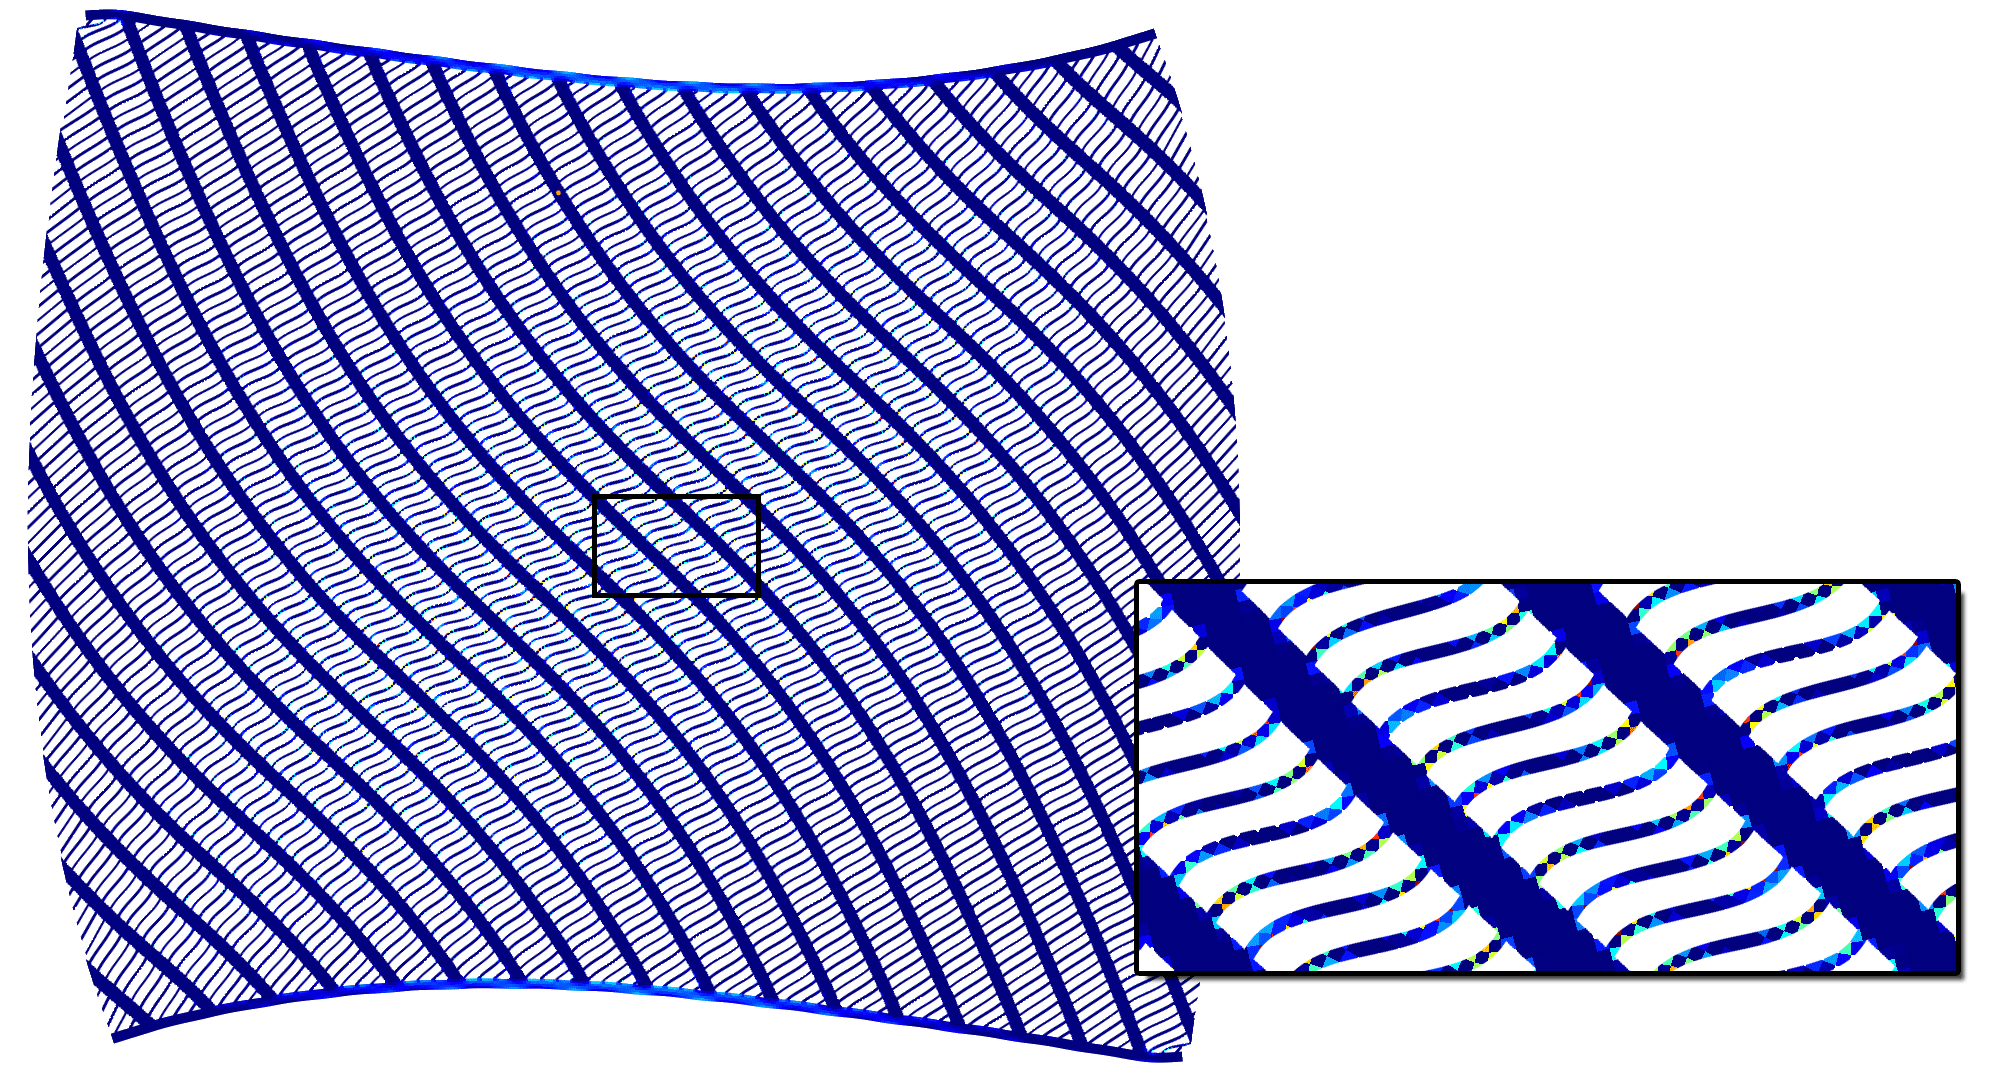
\includegraphics[width=.6\textwidth]{Images/two_scale.png}
    \caption{Macroscopic and microscopic length scales: notice that the
             deformation looks smooth when zoomed out (left), but when we zoom
             in on a few of the base cells, we see a periodic fluctuation
             in the displacement field. The original, undeformed object was a
             square, and a uniform squeezing force was applied to its top and
             bottom edges; if it weren't for its microstructure, the square
             would just contract uniformly in the vertical direction (an
             isotropic material with Poisson ratio 0 was used).}
    \label{fig:two_scale}
\end{figure}
By examining the deformation of a periodically tiled object under a particular
loading scenario, we see two distinct scales in the deformation field (see
Figure \ref{fig:two_scale}). This suggests that we use a two-scale analysis to
determine the macroscopic behavior as $\e \to 0$. We will end up with only a
heuristic derivation of the homogenized elasticity tensor, but once this tensor
is found it can be rigorously justified. The derivation here follows roughly
that in \cite{allaire2002shape} with some clarifications and added intuition.

For our two-scale analysis, we guess that the solution can be written as an asymptotic
expansion:
$$
{\bf u}^\e({\bf x}) = \sum_{p = 0}^{\infty} \e^p {\bf u}_p\left({\bf x}, \frac{{\bf x}}{\e}\right),
$$
with ${\bf u}_p({\bf x}, {\bf y})$ constrained to be $Y$-periodic in ${\bf y}$.
Each of these functions neatly separates its dependence on ${\bf x}$ (i.e. the
smoothly varying, macroscopic part) from its dependence on ${\bf y} = \frac{{\bf
x}}{\e}$ (the microscopic fluctuations) as suggested by Figure
\ref{fig:two_scale}. The periodicity constraint formalizes our insight that
the fluctuations are periodic (from Figure \ref{fig:two_scale}).

We plug this guess into the force balance equation (\ref{eqn:elastostatic}) and
equate coefficients of $\e^p$ on the left and right hand sides. We do this by
using the chain rule to compute each derivative:
$$
\tder{{\bf u}_p}{x_j} = \pder{{\bf u}_p}{x_j} + \frac{1}{\e} \pder{{\bf u}_p}{y_j}.
$$
Letting $\nabla_{\bf x}$ and $\nabla_{\bf y}$ be the vectors of differentiation
operators with respect to the macroscopic variables and microscopic variables
respectively, the force balance equation becomes, by linearity,

$$
-\sum_{p = 0}^\infty \e^p \left(\nabla_{\bf x} + \frac{1}{\e} \nabla_{\bf y}\right)
    \cdot \left[C({\bf y}) : \left(e_{\bf x}({\bf u}_p) + \frac{1}{\e} e_{\bf y}({\bf u}_p) \right) \right]
    = {\bf f}({\bf x}) \quad \text{in } \Omega,
$$
where $e_{\bf x}({\bf u}) = \frac{1}{2} \left( \nabla_{\bf x} {\bf u} + (\nabla_{\bf x}
{\bf u})^T \right)$ is the macroscopic strain operator, and $e_{\bf y}({\bf u}) =
\frac{1}{2} \left( \nabla_{\bf y} {\bf u} + (\nabla_{\bf y} {\bf u})^T \right)$
is the microscopic strain operator. Expanding, we get:
$$
-\sum_{p = 0}^\infty \e^p \nabla_{\bf x} \cdot [C({\bf y}) : e_{\bf x}({\bf u}_p)] +
\e^{p - 1} \left(\nabla_{\bf x} \cdot [C({\bf y}) : e_{\bf y}({\bf u}_p)] +
                 \nabla_{\bf y} \cdot [C({\bf y}) : e_{\bf x}({\bf u}_p)] \right) +
                 \e^{p - 2} \nabla_{\bf y} \cdot [C({\bf y}) : e_{\bf y}({\bf u}_p)] = {\bf f}
$$
This means the three lowest order equations in $\e$ are:
\begin{align}
    \e^{-2}:\quad  &-\nabla_{\bf y} \cdot [C({\bf y}) : e_{\bf y}({\bf u}_0)] = {\bf 0} \label{eqn:em2} \\
    \e^{-1}:\quad  &-\nabla_{\bf y} \cdot [C({\bf y}) : e_{\bf y}({\bf u}_1)] - 
                     \nabla_{\bf x} \cdot [C({\bf y}) : e_{\bf y}({\bf u}_0)] -
                     \nabla_{\bf y} \cdot [C({\bf y}) : e_{\bf x}({\bf u}_0)] = {\bf 0} \label{eqn:em1} \\
    \e^{ 0}:\quad  &-\nabla_{\bf y} \cdot [C({\bf y}) : e_{\bf y}({\bf u}_2)] - 
                     \nabla_{\bf x} \cdot [C({\bf y}) : e_{\bf y}({\bf u}_1)] -
                     \nabla_{\bf y} \cdot [C({\bf y}) : e_{\bf x}({\bf u}_1)] -
                     \nabla_{\bf x} \cdot [C({\bf y}) : e_{\bf x}({\bf u}_0)] = {\bf f} \label{eqn:e0}
\end{align}
We notice immediately that a function of the form ${\bf u}_0({\bf x}, {\bf y}) = {\bf u}({\bf x})$
(independent of ${\bf y}$) satisfies (\ref{eqn:em2}). The Fredholm alternative
proves that this solution is unique \cite[Lemma 2.3.21]{allaire2002shape}, but
this result is intuitive: (\ref{eqn:em2}) is effectively a force balance
equation for ${\bf u}_0$ in each instance of the periodic cell (i.e., at each
point ${\bf x}$). As boundary conditions, ${\bf u}_0$ is required to be
periodic in ${\bf y}$. This pins down the (infinitesimal) rotational degrees of
freedom, and all that remains is the translational degree of freedom: a
function ${\bf u}({\bf x})$ independent of ${\bf y}$. This ${\bf u}({\bf x})$ ends up
being the macroscopic displacement, as we will soon see.

Plugging in ${\bf u}({\bf x})$ for ${\bf u}_0$ simplifies (\ref{eqn:em1}) to:
\begin{equation}
    \label{eqn:u1u}
    -\nabla_{\bf y} \cdot (C({\bf y}) : [e_{\bf y}({\bf u}_1) + e_{\bf x}({\bf u})]) =  {\bf 0},
\end{equation}
where we used linearity to collect the strain terms. This equation yields a
unique solution for ${\bf u}_1({\bf x}, {\bf y})$ at each point ${\bf x}$ up to
a constant once ${\bf u}$ is known. Notice also that it is linear in $e_{\bf
x}({\bf u})$, so if we find ${\bf u}_1$ for each of 6 sample ${\bf u}({\bf x})$
carefully chosen so that their (macroscopic) strains span the 6-dimensional
space of strain tensors, then we can find ${\bf u}_1$ for any ${\bf u}$ by
superposition.

${\bf u}_1({\bf x}, {\bf y})$ and (\ref{eqn:u1u}) itself have a nice physical
interpretation: when we impose a smooth, macroscopic deformation on an object
as in Figure \ref{fig:two_scale}, the microstructure itself won't, in general,
be in equilibrium. Instead, there will be periodically fluctuating residual
forces, and we must superimpose a periodic microscopic fluctuation displacement
to balance them. For a particular macroscopic displacement ${\bf u}({\bf x})$,
force balance equation (\ref{eqn:u1u}) solves for this displacement.

Finally, we consider the $\e^0$ equation that ties everything together.
Grouping the strain terms, we get:
$$
 -\nabla_{\bf y} \cdot [C({\bf y}) : e_{\bf y}({\bf u}_2)] = 
                     \nabla_{\bf y} \cdot [C({\bf y}) : e_{\bf x}({\bf u}_1)] +
                     \nabla_{\bf x} \cdot (C({\bf y}) : [e_{\bf y}({\bf u}_1) + e_{\bf x}({\bf u})]) + {\bf f}
$$
We actually don't care about the value of ${\bf u}_2$, just that it exists and
is unique. This well-posedness requirement actually pins down the macroscopic
displacement ${\bf u}$. To see this, we average both sides of the equation
over the base cell $Y$ at each point ${\bf x}$:
$$
-\int_Y \! \nabla_{\bf y} \cdot [C({\bf y}) : e_{\bf y}({\bf u}_2)] \, \mathrm{d}{\bf y} = 
         \int_Y \!   \nabla_{\bf y} \cdot [C({\bf y}) : e_{\bf x}({\bf u}_1)] +
         \nabla_{\bf x} \cdot (C({\bf y}) : [e_{\bf y}({\bf u}_1) + e_{\bf x}({\bf u})]) + {\bf f} \, \mathrm{d} {\bf y}
$$
Applying the divergence theorem for the ${\bf y}$ variables:
$$
-\int_{\partial Y} \! [C({\bf y}) : e_{\bf y}({\bf u}_2)] {\bf \hat{n}} \, \mathrm{d}A({\bf y}) =
 \int_{\partial Y} \! [C({\bf y}) : e_{\bf x}({\bf u}_1)] {\bf \hat{n}} \, \mathrm{d}A({\bf y}) +
         \int_Y \nabla_{\bf x} \cdot (C({\bf y}) : [e_{\bf y}({\bf u}_1) + e_{\bf x}({\bf u})]) + {\bf f} \, \mathrm{d} {\bf y}
$$
Periodicity of $C({\bf y}) : e_{\bf y}({\bf u}_2)$ (both $C$ and ${\bf
u}_2$ are periodic in ${\bf y}$) means that the left-hand side is ${\bf 0}$.
Likewise, periodicity of ${\bf u}_1$ in ${\bf y}$ means $C({\bf y}) : e_{\bf x}({\bf
u}_1({\bf x}, {\bf y}))$ is also periodic in ${\bf y}$, so the surface integral
term on the right-hand side is ${\bf 0}$ as well. Thus, for a solution ${\bf
u}_2$ to exist, we must have:

$$
{\bf 0} = \int_Y \nabla_{\bf x} \cdot (C({\bf y}) : [e_{\bf y}({\bf u}_1) + e_{\bf x}({\bf u})]) + {\bf f} \, \mathrm{d} {\bf y}
$$
Exchanging the ${\bf x}$ divergence with the ${\bf y}$ integration, and pulling
out ${\bf f}$ (constant wrt. $y$) this equation becomes:
\begin{equation}
\label{eqn:almost_force_balance}
-\nabla_{\bf x} \cdot \int_Y C({\bf y}) : [e_{\bf y}({\bf u}_1) + e_{\bf x}({\bf u})] \, \mathrm{d} {\bf y} = |Y| {\bf f}
\end{equation}
This is starting to look like another force balance equation! Recall that ${\bf
u}_1$, up to a constant, depends linearly on $e_{\bf x}({\bf u})$ (see
(\ref{eqn:u1u})), which means that $e_{\bf y}({\bf u}_1)$ is a unique linear
function of $e_{\bf x}({\bf u})$. We can express this relationship with a rank
4 tensor ``$F$'' mapping macroscopic strain to microscopic fluctuation strain.
This allows us to make several simplifications:
$$
C({\bf y}) : [e_{\bf y}({\bf u}_1) + e_{\bf x}({\bf u})] = 
C({\bf y}) : [F : e_{\bf x}({\bf u}) + e_{\bf x}({\bf u})] = 
[C({\bf y}): F + C({\bf y})] : e_{\bf x}({\bf u}),
$$
where $[C({\bf y}) : F]_{ijkl} = C_{ijpq}({\bf y}) F_{pqkl}$ is the double
contraction of two rank 4 tensors. Using this in
(\ref{eqn:almost_force_balance}) and pulling out $e_{\bf x}({\bf u})$ (constant
wrt. ${\bf y}$) from the integral, we arrive at:
$$
-\nabla_{\bf x} \cdot \left( \frac{1}{|Y|} \int_Y C({\bf y}) : F + C({\bf y}) \, \mathrm{d} {\bf y} : e_{\bf x}({\bf u}) \right) = {\bf f}
$$
Setting, $C^H = \frac{1}{|Y|} \int_Y C({\bf y}) : F + C({\bf y}) \, \mathrm{d}
{\bf y}$, we finally have our homogenized force balance equation:
\begin{equation}
    \label{eqn:homogenized}
    -\nabla_{\bf x} \cdot [C^H : e_{\bf x}({\bf u}) ] = {\bf f} \quad \text{in } \Omega.
\end{equation}
Notice that we've only considered the force balance in the interior of $\Omega$
and haven't considered the boundary conditions in (\ref{eqn:elastostatic}). It
turns out that these boundary conditions don't affect $C^H$ (i.e. we get the same
homogenized elasticity tensor regardless of how we intend to deform the object)
\cite[Remark 3.1]{defranceschi1993}.

\subsection{Cell Problems}
All that remains is to use (\ref{eqn:u1u}) to determine rank 4 tensor $F$
appearing in $C^H$. First we introduce the canonical basis for symmetric rank 2 tensors:
$$
e^{ij} = \frac{1}{2} \left({\bf e}_i \otimes {\bf e}_j + {\bf e}_j \otimes {\bf e}_i \right)
$$
where ${\bf e}_i$ is the $i^\text{th}$ canonical basis element.
The 6 tensors $e^{ij}$ where $i \le j$ form a form a basis for the symmetric rank 2 tensors:
\begin{gather*}
e^{00} =
\begin{pmatrix}
        1 & 0 & 0 \\
        0 & 0 & 0 \\
        0 & 0 & 0
\end{pmatrix},\,
e^{11} =
\begin{pmatrix}
        0 & 0 & 0 \\
        0 & 1 & 0 \\
        0 & 0 & 0
\end{pmatrix},\,
e^{22} =
\begin{pmatrix}
        0 & 0 & 0 \\
        0 & 0 & 0 \\
        0 & 0 & 1
\end{pmatrix}, \\
e^{01} =
\begin{pmatrix}
        0 & 0.5 & 0 \\
        0.5 & 0 & 0 \\
        0 & 0 & 0
\end{pmatrix},\,
e^{02} =
\begin{pmatrix}
        0 & 0 & 0.5 \\
        0 & 0 & 0 \\
        0.5 & 0 & 0
\end{pmatrix},\,
e^{12} =
\begin{pmatrix}
        0 & 0 & 0 \\
        0 & 0 & 0.5 \\
        0 & 0.5 & 0
\end{pmatrix},
\end{gather*}
and the remaining 3 $e^{ij}$ with $i > j$ are equal to $e^{ji}$.

Then we can trivially expand the macroscopic strain at any point in this basis:
$$
e_{\bf x}({\bf u}) = e^{ij} [e_{\bf x}({\bf u})]_{ij}
$$

We now take advantage of linearity to state that if Y-periodic ${\bf
w}^{ij}({\bf y})$ solves (\ref{eqn:u1u}) for $e_{\bf x}({\bf u}) = e^{ij}$:
\begin{equation}
-\nabla_{\bf y} \cdot (C({\bf y}) : [e_{\bf y}({\bf w}^{ij}) + e^{ij}]) = {\bf 0},
\end{equation}
then ${\bf u}_1 = {\bf w}^{ij} [e_{\bf x}({\bf u})]_{ij}$ is a solution to
(\ref{eqn:u1u}) for arbitrary ${\bf u}$:
$$
-\nabla_{\bf y} \cdot (C({\bf y}) : [e_{\bf y}({\bf w}^{ij})[e_{\bf x}({\bf u})]_{ij} + e^{ij}[e_{\bf x}({\bf u})]_{ij}]) =
\left(-\nabla_{\bf y} \cdot (C({\bf y}) : [e_{\bf y}({\bf w}^{ij}) + e^{ij}]) \right)[e_{\bf x}({\bf u})]_{ij} = {\bf 0}.
$$
Since this solution is unique up to a constant wrt. ${\bf y}$, we know that
$$
e_{\bf y}({\bf u}_1) = e_{\bf y}({\bf w}^{ij} [e_{\bf x}({\bf u})]_{ij}) = e_{\bf y}({\bf w}^{ij})[e_{\bf x}({\bf u})]_{ij},
$$
which gives us the linear map from $e_{\bf x}({\bf u})$ to $e_{\bf y}({\bf u}_1)$
that $F_{pqkl}$ is meant to implement:
\begin{gather*}
e_{\bf y}({\bf u}_1) = F : e_{\bf x}({\bf u}) = e_{\bf y}({\bf w}^{kl})[e_{\bf x}({\bf u})]_{kl} \quad \Longrightarrow \\
[e_{\bf y}({\bf u}_1)]_{pq} = F_{pqkl} [e_{\bf x}({\bf u})]_{kl} = [e_{\bf y}({\bf w}^{kl})]_{pq}[e_{\bf x}({\bf u})]_{kl} \quad \Longrightarrow \\
F_{pqkl} = [e_{\bf y}({\bf w}^{kl})]_{pq}
\end{gather*}
Plugging this into the equation for the homogenized elasticity coefficients, we get in index notation:
\begin{equation}
    \label{eqn:Eh}
C^H_{ijkl} = \frac{1}{|Y|} \int_Y C_{ijpq}({\bf y}) F_{pqkl} + C_{ijkl}({\bf y}) \, \mathrm{d} {\bf y}
= \boxed{\frac{1}{|Y|} \int_Y C_{ijpq}({\bf y}) [e_{\bf y}({\bf w}^{kl})]_{pq} + C_{ijkl}({\bf y}) \, \mathrm{d} {\bf y}.}
\end{equation}
Thus, once we know each ${\bf w}^{ij}$, we can compute the homogenized elasticity tensor
with a simple integration over the base cell. We find these by solving the 6 cell problems:
\begin{align*}
    -\nabla_{\bf y} \cdot (C({\bf y}) : [e_{\bf y}({\bf w}^{ij}) + e^{ij}]) = {\bf 0} & \quad \text{in } Y \\
    {\bf w}^{ij}({\bf y})\ Y \text{-periodic} &     \numberthis \label{eqn:cell} \\
    \int_\omega \! {\bf w}^{ij}({\bf y})  \, \mathrm{d} {\bf y} =  {\bf 0}, 
\end{align*}
one for each canonical basis tensor $e^{ij}$. The last constraint is to pin
down the remaining translational degree of freedom; since we only care about
strain $e_{\bf y}({\bf w}^{ij})$, we can arbitrarily choose to enforce ${\bf
0}$ average displacement over the microstructure geometry.

Intuitively, solving each cell problem (\ref{eqn:cell}) corresponds to probing
the base cell with 6 constant strain displacements to extract how the
microstructure geometry $\omega$ reacts (i.e. the fluctuation displacements).
Then the homogenized elasticity tensor given in (\ref{eqn:Eh}) corresponds to a
spatial average of $C({\bf y})$ corrected by the fluctuation terms (which
happen to be averaged fluctuation stresses). We can get a more physical
interpretation of (\ref{eqn:Eh}) by realizing that it is equivalent to:
\begin{equation}
    \label{eqn:EhEnergy}
    C^H_{ijkl} = \frac{1}{|Y|} \int_Y (e^{ij} + e_{\bf y}({\bf w}^{ij})) : C({\bf y}) : (e^{kl} + e_{\bf y}({\bf w}^{kl})) \, \mathrm{d} {\bf y}.
\end{equation}
This means that when we use the homogenized elasticity tensor to compute the
elastic energy density stored at point ${\bf x}$ by some macroscopic strain
$\bar{e}$,
$$
\frac{1}{2} (\bar{e} : C^H :\bar{e}) =
\frac{1}{2|Y|} \int_Y \bar{e}_{ij} (e^{ij} + e_{\bf y}({\bf w}^{ij})) : C({\bf y}) : (e^{kl} + e_{\bf y}({\bf w}^{kl})) \bar{e}_{kl} \, \mathrm{d} {\bf y},
$$
what we get is the average energy density stored by the macroscopic strain plus
its fluctuation strain. Proof of this equivalence: start with RHS of
(\ref{eqn:EhEnergy}) and work backward.
\begin{gather*}
\frac{1}{|Y|} \int_Y (e^{ij} + e_{\bf y}({\bf w}^{ij})) : C({\bf y}) : (e^{kl} + e_{\bf y}({\bf w}^{kl})) \, \mathrm{d} {\bf y} \\
= \frac{1}{|Y|} \int_Y e^{ij} : C({\bf y}) : (e^{kl} + e_{\bf y}({\bf w}^{kl})) +
    e_{\bf y}({\bf w}^{ij}) : C({\bf y}) : (e^{kl} + e_{\bf y}({\bf w}^{kl})) \, \mathrm{d} {\bf y} \\
    = \frac{1}{|Y|} \int_Y C_{ijpq}({\bf y}) [e^{kl} + e_{\bf y}({\bf w}^{kl})]_{pq} -
{{\bf w}}^{ij} \cdot \cancel{\nabla_y \cdot [C({\bf y}) : (e^{kl} + e_{\bf y}({\bf w}^{kl}))]} \, \mathrm{d} {\bf y} \\
+ \cancel{\int_{\partial Y} {\bf w}^{ij} \cdot [C({\bf y}) : (e^{kl} + e_{\bf y}({\bf w}^{kl}))] {\bf \hat{n}} \, \mathrm{d} A({\bf y})}
= \frac{1}{|Y|} \int_Y C_{ijpq}({\bf y}) [e_{\bf y}({\bf w}^{kl})]_{pq} + C_{ijkl}({\bf y}) \, \mathrm{d} {\bf y} = C^H_{ijkl}.
\end{gather*}
Here we used integration by parts (for symmetric tensors) to move the strain
operator off ${\bf w}^{ij}$. The resulting volume integral vanishes because ${\bf
w}^{kl}$ solves the $kl^\text{th}$ cell problem. The surface integral vanishes
because row vector ${\bf w}^{ij} \cdot [C({\bf y}) : (e^{kl} + e_{\bf
y}({\bf w}^{kl}))]$ is Y-periodic.

Notice that this periodicity only holds
in the continuous case where $e_{\bf y}({\bf w}^{kl})$ is periodic due to ${\bf
w}^{kl}$'s periodicity. When we discretize (with FEM) this no longer holds exactly.
However, notice that the term we want to vanish,
$ \frac{1}{|Y|} \int_Y e_{\bf y}({\bf w}^{ij}) : C({\bf y}) : (e^{kl} + e_{\bf y}({\bf w}^{kl})) \,
\mathrm{d} {\bf y}$, can be written as a linear combination of
$ \frac{1}{|Y|} \int_Y e_{\bf y}(\phi) : C({\bf y}) : (e^{kl} + e_{\bf y}({\bf
w}^{kl})) $
for basis functions $\phi$. For each $\phi$, we recognize this as a row of the
FEM system for the $kl^\text{th}$ cell problem, which will be exactly zero (up
to roundoff error). Thus the term does indeed vanish in the discrete case.

\section{Rigorous Justification}
The derivation is only a heuristic procedure, not a proof that that the
sequence of solutions ${\bf u}^\e$ approaches the solution to the
homogenized equation, ${\bf u}$, as $\e \to 0$ . To prove this requires a lot of mathematical
formalism, such as weak and H-/G-convergence. \cite{allaire2002shape} provides the details.

\section{Solving the Cell Problems}
The homogenization task has now been reduced to solving 6 cell problems:
\begin{align*}
    -\nabla \cdot (C({\bf y}) : [e({\bf w}^{ij}) + e^{ij}]) = {\bf 0} & \quad \text{in } Y \\
    {\bf w}^{ij}({\bf y})\ Y \text{-periodic} & \\
    \int_\omega \! {\bf w}^{ij}({\bf y})  \, \mathrm{d} {\bf y} =  {\bf 0}, 
\end{align*}
(from here on out we drop the ${\bf y}$ subscripts since only the ${\bf y}$
variables remain) and computing a volume integral:
$$
C^H_{ijkl} = \frac{1}{|Y|} \int_Y C_{ijpq}({\bf y}) [e({\bf w}^{kl})]_{pq} + C_{ijkl}({\bf y}) \, \mathrm{d} {\bf y}.
$$
Recalling that 
$$
C ({\bf y}) = \begin{cases} C^\text{base} & \text{if } {\bf y} \in \omega \\
                                 0 & \text{ otherwise,} \end{cases}
$$
we should be able to compute all of this with a single-material finite element discretization
of the microstructure pattern $\omega$ filling cell $Y$:
\begin{figure}[H]
    \centering
    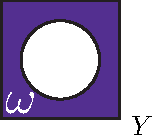
\includegraphics[width=.16\textwidth]{Images/cell.pdf}
\end{figure}
But now we see a problem: $C({\bf y})$ is discontinuous at microstructure boundary $\partial \omega \setminus \partial Y$. Also,
the cell problem isn't well-posed since ${\bf w}^{ij}({\bf y})$ can take any
value outside $\omega$. We can get around this by restricting the cell problem to $\omega$:
\begin{align*}
    -\nabla \cdot (C^\text{base} : [e({\bf w}^{ij}) + e^{ij}]) = {\bf 0} & \quad \text{in } \omega \\
    {\bf w}^{ij}({\bf y})\ Y \text{-periodic} & \\
    \int_\omega \! {\bf w}^{ij}({\bf y})  \, \mathrm{d} {\bf y} =  {\bf 0}, 
\end{align*}
(only solving for fluctuation displacements inside $\omega$). This is fine
since the homogenized elasticity tensor formula's integral also becomes an
integral over only $\omega$:
$$
C^H_{ijkl} = \frac{1}{|Y|} \int_\omega C_{ijpq}^\text{base} [e({\bf w}^{kl})]_{pq} + C_{ijkl}^\text{base} \, \mathrm{d} {\bf y}.
$$
However, we have the question of what boundary conditions to impose on
$\partial \omega \setminus \partial Y$. We show that the equivalent conditions
are actually a boundary traction balance, as might be suspected:

Consider an arbitrary smooth segment $\Gamma \subseteq \partial \omega \setminus
\partial Y$ (we assume
$\partial \omega$ is piecewise smooth and can be covered with these segments).
Create a small volume, $V_\xi$ by extruding in the $\pm \bf \hat{n}$ direction
by $\xi$. Letting $\sigma = C({\bf y}) : [e({\bf w}^{ij}) + e^{ij}]$, the
original cell problem formulation requires:
$$
0 = \int_{V_\xi} \! \nabla \cdot \sigma \, \mathrm{d} V
$$
Since $\nabla \cdot$ is invariant to orthogonal transformations, at each point
we can can rotate to align one of our coordinate axes with ${\bf \hat{n}}$ and write:
$$
\nabla \cdot \sigma = \pder{}{\bf \hat{n}}({\bf \hat n} \cdot \sigma)  + \nabla_{{\bf \hat n}^\perp} \cdot \sigma,
$$
where $\nabla_{{\bf \hat n}^\perp} \cdot \sigma$ takes the 2D divergence in the
directions perpendicular to ${\bf n}$ (i.e. tangent to the boundary). Because
$\sigma$ varies smoothly over $\Gamma$, these components of the divergence are
bounded. Thus, as $\xi \to 0$ (and $|V_\xi| \to 0$), these contributions to the
integral vanish and we have:
$$
0 = \lim_{\xi \to 0} \int_{V_\xi} \! \nabla \cdot \sigma \, \mathrm{d} V  =
    \lim_{\xi \to 0} \int_{V_\xi} \! \pder{}{\bf \hat{n}}({\bf \hat n} \cdot \sigma) \, \mathrm{d} V
$$
Since ${\bf \hat n} \cdot \sigma$ goes from ${\bf \hat n} \cdot \sigma({\bf
y}_\Gamma)$ at a point on $\Gamma$ immediately to $0$ just outside $\omega$
when traveling in the normal direction,
$$
\pder{}{\bf \hat{n}}({\bf \hat n} \cdot \sigma) =
-\delta_\Gamma({\bf y}) ({\bf \hat n} \cdot \sigma({\bf y})) + \text{bounded term}
$$
where $-\delta_\Gamma({\bf y})$ is 3D delta function that is nonzero everywhere
except on $\Gamma$ and whose 1D integral in the normal direction is 1. The bounded
term is for the derivative at points inside the object where $\sigma$ varies
smoothly. This term vanishes as $\xi \to 0$, so we are left with:
$$
0 = -\lim_{\xi \to 0} \int_{V_\xi} \! \delta_\Gamma({\bf y}) ({\bf \hat n} \cdot \sigma({\bf y})) \, \mathrm{d} V =
    -\lim_{\xi \to 0} \int_{\Gamma} \! {\bf \hat n} \cdot \sigma({\bf y}) \, \mathrm{d} A =
    -\int_{\Gamma} \! {\bf \hat n} \cdot \sigma({\bf y}) \, \mathrm{d} A
$$
Since $\Gamma$ was arbitrary, this means ${\bf \hat n} \cdot \sigma({\bf y}) = 0$
everywhere on $\partial \omega \setminus \partial Y$, giving us our full cell
problem:
\begin{align*}
     -\nabla \cdot (C^\text{base} : [e({\bf w}^{ij}) + e^{ij}]) = {\bf 0} & \quad \text{in } \omega \\
{\bf \hat n} \cdot (C^\text{base} : [e({\bf w}^{ij}) + e^{ij}]) = {\bf 0} & \quad \text{on } \partial \omega \setminus \partial Y \\
    {\bf w}^{ij}({\bf y})\ Y \text{-periodic} & \\
    \int_\omega \! {\bf w}^{ij}({\bf y})  \, \mathrm{d} {\bf y} =  {\bf 0}, 
\end{align*}

This is finally a well-posed force balance equation in $\omega$ that is
consistent with our interpretation of the cell problem as finding fluctuation
displacements that put the microstructure geometry in equilibrium after a
particular macroscopic strain has been applied.

Since macroscopic stress $C^\text{base} : e^{ij}$ is constant throughout the
base cell, we can actually write this as:
\begin{align*}
     -\nabla \cdot (C^\text{base} : e({\bf w}^{ij})]) = {\bf 0} & \quad \text{in } \omega \\
{\bf \hat n} \cdot \left[ C^\text{base} : e({\bf w}^{ij}) \right]  =  -{\bf \hat{n}} \cdot \left[ C^\text{base} : e^{ij} \right]& \quad \text{on } \partial \omega \setminus \partial Y \\
    {\bf w}^{ij}({\bf y})\ Y \text{-periodic} & \\
    \int_\omega \! {\bf w}^{ij}({\bf y})  \, \mathrm{d} {\bf y} =  {\bf 0}, 
\end{align*}
This highlights the fact that the volume force density in the original cell
problem formulation (\ref{eqn:cell}) is really zero everywhere except for delta
functions sitting on the microstructure boundary that end up becoming the
surface traction.

\subsection{FEM Implementation}
The cell problems are discretized and solved numerically using the finite
element method, which also leads to a discretization of the volume integral
to compute the homogenized elasticity coefficients. Notice that only a
single base cell of the geometry needs to be discretized, making the
computation very efficient.

Two FEM implementations are used: a traditional volume mesh discretization using
linear tetrahedron elements, and a novel ``mesh free'' method using a grid of
trilinear cubes not conforming to the object's boundary. The mesh free method is
nice for tasks such as shape/topology optimization where the object will change
frequently and remeshing is intractable--the method works directly on an
object's level set description (or any description allowing efficient
inside/outside tests).

The linear elasticity solver obviously needs to support periodic boundary
conditions. This is tricky for the tet-based solver because it requires the
microstructure geometry to be tessellated identically on opposite periodic cell
faces. The mesh free method is more forgiving in this regard: as long as the
geometry itself is periodic, the computation grid will always match up across
the periodic boundaries.

Periodic boundary conditions are implemented by direct elimination of
variables (reducing the size of the system); for microstructures filling large
portions of the periodic boundaries, the speedup and memory efficiency gained
by direct elimination over Lagrange multipliers is significant.
Direct elimination is performed by
assigning all mesh/grid nodes in each connected component of the ``identified
vertex graph'' the same degrees of freedom. For example, the cell's corner
nodes--if they exist--appear as the graphs only component of size 8 and all get
the same $x$, $y$, and $z$ displacement degrees of freedom. Edge nodes will
appear in a component of size 4.

In both cases, to simplify operations such as rank 4 tensor inversion (to get
the ``stress to strain'' compliance tensor from the ``strain to stress'' elasticity
tensor) and double contractions, we use a symmetric tensor flattening approach
to turn rank 4 tensors into matrices and rank 2 tensors into vectors. Since
care must be taken in this transformation, the approach is detailed in the
Tensor Flattening writeup. We end up storing the elasticity tensor as a
symmetric $6\times 6$ matrix with 21 coefficients.

\bibliographystyle{plain}
\bibliography{References}

\end{document}
